\documentclass[9pt,table,xcolor=dvipsnames]{beamer}
\input{Common-White.tex}
  \title{Analysis of Tetris Ballistic Deposition and the Robustness of the KPZ Universality Class}% {{{
% \subtitle
% {Research Plan} % (optional)

\author[Le Chen]{Le Chen\\
  Auburn University\\[2em]
  \footnotesize Acknwolegement\\[0.5em]
  \textit{NSF 2246850, NSF 2443823, \& Simons Foundation Travel Grant (2022-2027)}\\[1.3em]
  \href{https://chenle02.github.io/2025-10-28_Emerging_Synergies_Banff_Le/}{\texttt{Talk available at: github.com/chenle02}}%
% \small University of Cardiff \\[1.5em]
% https://chenle02.github.io/2025-10-28_Emerging_Synergies_Banff_Le/
}
% - Use the \inst{?} command only if the authors have different
%   affiliation.
\institute[Auburn University]
{%
% \pgfuseimage{Auburn}
% Jointwork with\\[1em]
% Raluca Balan, Xia Chen and Nicholas Eisenberg \\
 % \vspace{2cm}
 }
% - Use the \inst command only if there are several affiliations.
% - Keep it simple, no one is interested in your street address.

% \date[Talk at Karlsruhe] % (optional)
% {\today }
\date[Banff]{
{\small Emerging Synergies between Stochastic Analysis and Statistical Mechanics} \\
{\small Banff, Alberta, Canada} \\
{\small October 28, 2025}
}

% This is only inserted into the PDF information catalog. Can be left
% out.

% If you have a file called "university-logo-filename.xxx", where xxx
% is a graphic format that can be processed by latex or pdflatex,
% resp., then you can add a logo as follows:

% \pgfdeclareimage[height=2cm]{Auburn}{figs/AU-Black.jpeg}

% Delete this, if you do not want the table of contents to pop up at
% the beginning of each subsection:
% \AtBeginSubsection[]
% {
%   \begin{frame}<beamer>{Outline}
%     \tableofcontents[currentsection,currentsubsection]
%   \end{frame}
% }

% If you wish to uncover everything in a step-wise fashion, uncomment
% the following command:

% \beamerdefaultoverlayspecification{<+->}

\begin{document}

\begin{frame}[noframenumbering] % Title page.
  \titlepage
\end{frame}

\begin{frame}<15->{Motivation}
  \small  % slightly smaller text looks nicer on dense slides

  \begin{columns}[T,onlytextwidth]
    \column{0.55\textwidth}
    \begin{block}{Outreach}
      \begin{itemize}\itemsep2pt
        \item Auburn Summer Science Institute (AU-SSI): \textbf{2024, 2025}\\
              \emph{Selected talented high school students}
        \item Destination STEM: \textbf{2023, 2024}\\
              \emph{Junior middle school students}
        \item Graduate Student Seminars (Mathematics), Auburn: \textbf{2022--2025}
      \end{itemize}
    \end{block}

    \column{0.45\textwidth}
    \begin{block}{Teaching}
      \begin{itemize}\itemsep2pt
        \item \textbf{Math 7820/7830: Applied Stochastic Processes}\\
              Course project, \textbf{2023/24}
      \end{itemize}
    \end{block}

  \end{columns}
  \vfill
  \begin{center}
    Most materials are available at \\ \bigskip
    \href{https://github.com/chenle02/}{\texttt{github.com/chenle02}}%
  \end{center}
\end{frame}
\begin{frame}[fragile] % Coauthors
  \begin{center}
    Math 7820/30: Applied Stochastic Processes (2023/24):
    \includegraphics[scale=0.30]{./figs/mau.jpeg}
    \includegraphics[scale=0.50]{./figs/ruau.jpg}
    \bigskip

    Mauricio Montes and Ian Ruau
  \end{center}
\end{frame}
\begin{frame}[fragile,t] % COMENTS
  \begin{center}
    \includegraphics[scale=0.20]{./figs/Contrasting_Sand_and_Snow_Pile.png}
    \bigskip

    \small Image is generated by OpenAI's \textit{DALL-E} 

  \end{center}
\end{frame}
\begin{frame}{Plan} % TOC
 \tableofcontents
\end{frame}
\section{Introduction to growth model and SPDE}
\begin{frame}[fragile] % Random deposition
  \frametitle{Random deposition}

  \begin{center}
    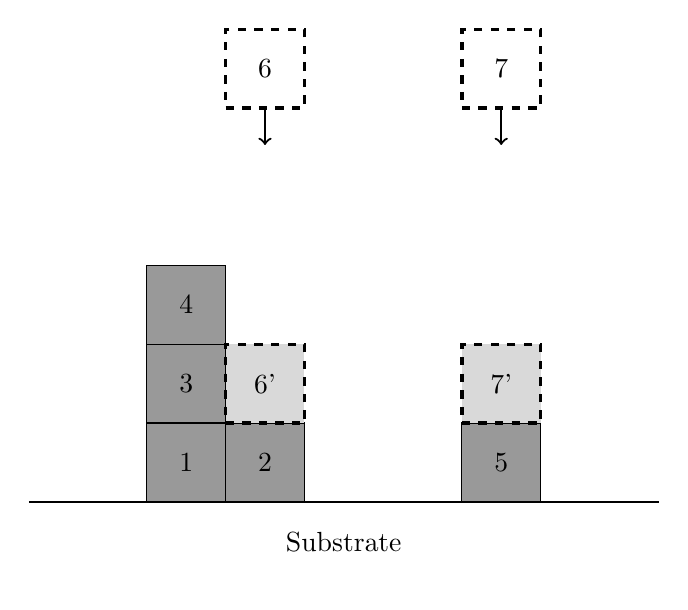
\begin{tikzpicture}[every node/.style={draw, minimum size=1cm}, node distance=0cm]
      \tikzset{
        solidnode/.style={draw, fill = gray!80!white, solid, minimum size=1cm},
        dashnodeX/.style={
          draw, dashed, minimum size=1cm, very thick,
          append after command={
            (\tikzlastnode.south) [shorten >=1.5pt, very thick] edge [->, thick] ++(0,-0.5cm)
          }
        },
        dashnodeD/.style={draw, dashed, minimum size=1cm, very thick, fill = gray!30!white},
      }
      \draw[thick] (0,-0.5) --++ (8,0) node [midway, below, draw=none] {Substrate};
      \node[solidnode] (1) at (2,0) {1};
      \node[solidnode] (3) at (2,1) {3};
      \node[solidnode] (4) at (2,2) {4};
      \node[solidnode] (5) at (3,0) {2};
      \node[solidnode] (2) at (6,0) {5};

      \pause
      \node[dashnodeX] (6) at (3,5) {6};
      \node[dashnodeX] (7) at (6,5) {7};

      \pause
      \node[dashnodeD] (6') at (3,1) {6'};

      \pause
      \node[dashnodeD] (7') at (6,1) {7'};
    \end{tikzpicture}
  \end{center}

\end{frame}

\begin{frame}[fragile] % Random deposition with surface relaxation.
  \frametitle{Random deposition with surface relaxation}

  \begin{center}
    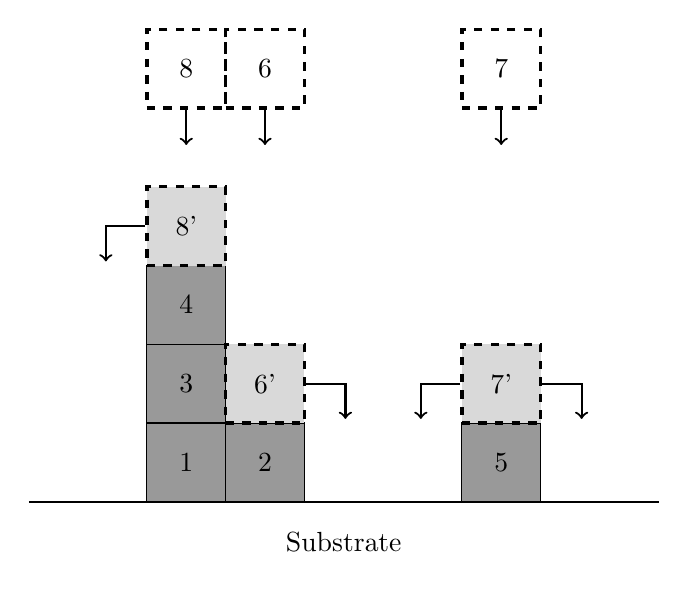
\begin{tikzpicture}[every node/.style={draw, minimum size=1cm}, node distance=0cm]
      \tikzset{
        solidnode/.style={
            draw, fill=gray!80!white, solid, minimum size=1cm
        },
        dashnodeX/.style={
            draw, dashed, minimum size=1cm, very thick,
            append after command={
            \pgfextra{  % the \pgfextra command allows multiple draw commands
                \draw [->, thick, shorten >=1.5pt] (\tikzlastnode.south) -- ++(0,-0.5cm);
                % \draw [->, thick, shorten <=1.5pt] (\tikzlastnode.north) -- ++(0,0.5cm);
            }
            }
        },
        dashnodeR/.style={
            draw, dashed, minimum size=1cm, very thick, fill=gray!30!white,
            append after command={
            \pgfextra{  % the \pgfextra command allows multiple draw commands
                \draw [->, thick, shorten >=1.5pt] (\tikzlastnode.east) -- ++(0.5cm,0) -- ++(0,-0.5cm);
                % \draw [->, thick, shorten <=1.5pt] (\tikzlastnode.north) -- ++(0,0.5cm);
            }
            }
        },
        dashnodeL/.style={
            draw, dashed, minimum size=1cm, very thick, fill=gray!30!white,
            append after command={
            \pgfextra{  % the \pgfextra command allows multiple draw commands
                \draw [->, thick, shorten >=1.5pt] (\tikzlastnode.west) -- ++(-0.5cm,0) -- ++(0,-0.5cm);
                % \draw [->, thick, shorten <=1.5pt] (\tikzlastnode.north) -- ++(0,0.5cm);
            }
            }
        },
        dashnodeT/.style={
            draw, dashed, minimum size=1cm, very thick, fill=gray!30!white,
            append after command={
            \pgfextra{  % the \pgfextra command allows multiple draw commands
                \draw [->, thick, shorten >=1.5pt] (\tikzlastnode.east) -- ++(0.5cm,0) -- ++(0,-0.5cm);
                \draw [->, thick, shorten >=1.5pt] (\tikzlastnode.west) -- ++(-0.5cm,0) -- ++(0,-0.5cm);
                % \draw [->, thick, shorten <=1.5pt] (\tikzlastnode.north) -- ++(0,0.5cm);
            }
            }
        }
      }
      \draw[thick] (0,-0.5) --++ (8,0) node [midway, below, draw=none] {Substrate};
      \node[solidnode] (1) at (2,0) {1};
      \node[solidnode] (3) at (2,1) {3};
      \node[solidnode] (4) at (2,2) {4};
      \node[solidnode] (5) at (3,0) {2};
      \node[solidnode] (2) at (6,0) {5};

      \pause
      \node[dashnodeX] (6) at (3,5) {6};
      \node[dashnodeX] (7) at (6,5) {7};
      \node[dashnodeX] (8) at (2,5) {8};

      \pause
      \node[dashnodeR] (6') at (3,1) {6'};

      \pause
      \node[dashnodeT] (7') at (6,1) {7'};

      \pause
      \node[dashnodeL] (8') at (2,3) {8'};
    \end{tikzpicture}
  \end{center}
\end{frame}
\begin{frame}[fragile] % Ballistic deposition with surface relaxation.
  \frametitle{Ballistic deposition}

  \begin{center}
    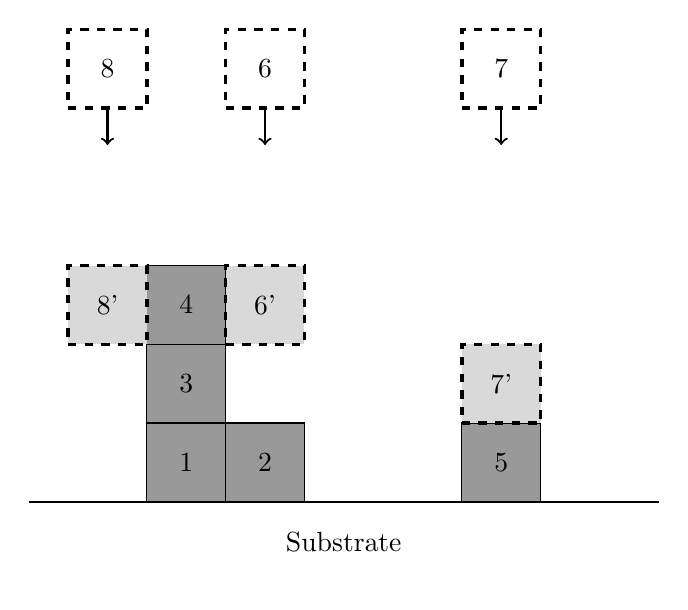
\begin{tikzpicture}[every node/.style={draw, minimum size=1cm}, node distance=0cm]
      \tikzset{
        solidnode/.style={
            draw, fill=gray!80!white, solid, minimum size=1cm
        },
        dashnodeX/.style={
            draw, dashed, minimum size=1cm, very thick,
            append after command={
            \pgfextra{  % the \pgfextra command allows multiple draw commands
                \draw [->, thick, shorten >=1.5pt] (\tikzlastnode.south) -- ++(0,-0.5cm);
                % \draw [->, thick, shorten <=1.5pt] (\tikzlastnode.north) -- ++(0,0.5cm);
            }
            }
        },
        dashnodeD/.style={draw, dashed, minimum size=1cm, very thick, fill = gray!30!white},
      }
      \draw[thick] (0,-0.5) --++ (8,0) node [midway, below, draw=none] {Substrate};
      \node[solidnode] (1) at (2,0) {1};
      \node[solidnode] (3) at (2,1) {3};
      \node[solidnode] (4) at (2,2) {4};
      \node[solidnode] (5) at (3,0) {2};
      \node[solidnode] (2) at (6,0) {5};

      \pause
      \node[dashnodeX] (6) at (3,5) {6};
      \node[dashnodeX] (7) at (6,5) {7};
      \node[dashnodeX] (8) at (1,5) {8};

      \pause
      \node[dashnodeD] (6') at (3,2) {6'};

      \pause
      \node[dashnodeD] (7') at (6,1) {7'};

      \pause
      \node[dashnodeD] (8') at (1,2) {8'};
    \end{tikzpicture}
  \end{center}
\end{frame}
\begin{frame}[fragile] % Average height and fluctuation
  \frametitle{Average height and fluctuation}
   \begin{center}
     \begin{tikzpicture}[every node/.style={draw, minimum size=1cm}, node distance=0cm]
      \tikzset{
        solidnode/.style={
            draw, fill=gray!80!white, solid, minimum size=1cm
        },
        dashnodeX/.style={
            draw, dashed, minimum size=1cm, very thick,
            append after command={
            \pgfextra{  % the \pgfextra command allows multiple draw commands
                \draw [->, thick, shorten >=1.5pt] (\tikzlastnode.south) -- ++(0,-0.5cm);
                % \draw [->, thick, shorten <=1.5pt] (\tikzlastnode.north) -- ++(0,0.5cm);
            }
            }
        },
        dashnodeD/.style={draw, dashed, minimum size=1cm, very thick, fill = gray!30!white},
      }
      \draw[thick] (-0.5,-0.5) --++ (8,0) node [midway, below, draw=none, yshift = -1em] {Substrate size $L=8$}; % node [right, draw = none, xshift =-1em] {$x$};
      \draw[thick] (-0.5,-0.5) --++ (0,4);
      \draw[thick] (+7.5,-0.5) --++ (0,4);
      \draw[thick, ->] (-1.2,-1.0) --++ (0,5) node [above, draw = none] {$h(8,x) = $};
      \foreach \y in {0,1,...,4}{
        \draw[thick] (-1.1,\y-1) --++ (-0.2,0) node [left, draw = none, xshift = 0em] {\y};
      }

      \foreach \x in {1,...,8}{
        \draw[thick] (\x-1,-0.5) --++ (0,-0.1) node [below, draw = none, yshift = 1em] {\x};
        \draw[dotted] (\x-0.5,-0.5) --++ (0,4);
      }
      \node[draw = none] at (0, 4.5) {0};
      \node[draw = none] at (1, 4.5) {3};
      \node[draw = none] at (2, 4.5) {3};
      \node[draw = none] at (3, 4.5) {3};
      \node[draw = none] at (4, 4.5) {0};
      \node[draw = none] at (5, 4.5) {0};
      \node[draw = none] at (6, 4.5) {2};
      \node[draw = none] at (7, 4.5) {0};

      \node[solidnode] (1) at (2,0) {1};
      \node[solidnode] (3) at (2,1) {3};
      \node[solidnode] (4) at (2,2) {4};
      \node[solidnode] (5) at (3,0) {2};
      \node[solidnode] (2) at (6,0) {5};
      \node[solidnode] (6) at (3,2) {6};
      \node[solidnode] (7) at (6,1) {7};
      \node[solidnode] (8) at (1,2) {8};

      \only<2->{
        \draw[thick, dashed] (-0.7, 11/8 - 1) --++ (8.4,0) node[right, draw = none] {$\overline{h}(8) = \dfrac{11}{8}$};
        \node[draw = none] (av) at (-0.5,6) {$ \displaystyle \overline{h}(t) = \frac{1}{L}\sum_{x=1}^{L}h(t,x)$};
        \node[draw = none] (fl) at (5,6.0) {Fluctuation $ \displaystyle W(L,t) = \sqrt{\frac{1}{L}\sum_{x=1}^{L}\left[h(t,x) - \overline{h}(t)\right]^2}$};
      }

      \only<3->{
        \draw[red, thick] (0,-1) -- (1,2) -- (2,2) -- (3,2) -- (4,-1) -- (5,-1) -- (6, 1) -- (7,-1);
      }

    \end{tikzpicture}
  \end{center}
\end{frame}

\begin{frame}[t]{Random Deposition (independent columns, nonsticky)}
  \small \textbf{Model.} $L$ independent columns. At each integer time $t =
  1,2,\dots$, drop \emph{one} particle on a uniformly random column. Heights
  $h(t,x)$, mean $\overline h(t)=\frac1L\sum_{x=1}^L h(t,x) = \frac{t}{L}$,
  width
  \[
    W^2(L,t)=\frac1L\sum_{x=1}^L \big(h(t,x)-\overline h(t)\big)^2.
  \]

  \pause\medskip\textbf{Single--column law:} After $t$ drops total,
  \[
    h(t,x)\sim \mathrm{Binomial}\!\left(t,\frac1L\right),\qquad
    \mathbb E[h(t,x)]=\frac{t}{L},\quad \mathrm{Var}(h(t,x))=\;t\,\frac1L\!\left(1-\frac1L\right).
  \]

  \pause\medskip\textbf{Fluctuation:} By i.i.d.\ columns,
  \[
    \mathbb E\!\left[W^2(L,t)\right]
    =\frac1L\sum_{x=1}^L\mathbb E\left[h(t,x)^2\right] - \mathbb E\left[\overline h^{\,2}(t)\right]
    =\mathbb E\left[h(t,1)^2\right] - \left(\frac{t}{L}\right)^2
    =\left(1-\frac1L\right) \mathrm{Var}\!\big(h(t,1)\big).
  \]
  Hence
  \[
    \boxed{\;\mathbb E\!\left[W^2(L,t)\right]
    =\Big(1-\frac1L\Big)\,t\,\frac1L\!\left(1-\frac1L\right)
    =\frac{t}{L}\left(1-\frac1L\right)^{\!2}\;}
  \]
  and
  \[
    \boxed{\,W(L,t)\; \simeq \;\left(1-\frac1L\right)\;\left(\frac{t}{L}\right)^{1/2}\,}
  \]

  \medskip \alert{Scaling.} Growth exponent \( \displaystyle \beta = \frac12\).
  % \(W^2(L,t)\simeq t/L\) (no lateral correlations, no true saturation).

\end{frame}
\begin{frame}[fragile] % COMENTS
  For ballistic deposition (sticky), lateral interactions appear, can we view it
  as a perturbation of random deposition (nonsticky)?
\end{frame}
\begin{frame}[fragile] % Random diposition vs ballistic decomposition
  \begin{center}
    \Large Simulations on \\ \bigskip
    Random deposition vs. Ballistic decomposition
  \end{center}
\end{frame}
\begin{frame}[fragile] % More models
  \frametitle{More models? Even more simpler?}

  \begin{center}
    \begin{tikzpicture}
        % Node for the image
        \node[anchor=east, inner sep=0] (image) at (0,0) {\includegraphics[width=0.5\textwidth]{./figs/Figure_8-4_SOS-Issing-Gas.png}};

        % Labels
        \node[anchor=west] at ([yshift=3cm]image.east) {Solid-on-Solid};
        \node[anchor=west] at ([yshift=1.4cm]image.east) {Ising};
        \node[anchor=west] at ([yshift=0.8cm]image.east) {Lattice Gas};
    \end{tikzpicture}
  \end{center}

\end{frame}
\begin{frame}[fragile] % Paper -- a random environment
  \frametitle{Paper -- a random environment}

  \begin{center}
    \includegraphics[scale=0.20]{./figs/Paper_Random_Environment.png}
  \end{center}

  \myFootCite{zhang.zhang.ea:92:modeling}
\end{frame}
\begin{frame}[fragile] % Paper wetting experiments
  \frametitle{Paper wetting experiment}

  \begin{center}
    \includegraphics[scale=0.14]{./figs/Figure_1-2_Paper-ink.png} \pause
    \includegraphics[scale=0.20]{./figs/Figure_1-2_PaperInk-b-c.png}
  \end{center}

  \myFootCite{barabasi.stanley:95:fractal}
\end{frame}
\begin{frame}[fragile] % Paper burning experiment
  \frametitle{Paper burning experiment}

  \begin{center}
    \includegraphics[scale=0.25]{./figs/Figure_1-3_Paper_Fire.png}
  \end{center}

  \myFootCite{zhang.zhang.ea:92:modeling}
\end{frame}
\begin{frame}[fragile] % Paper rupture experiments
  \frametitle{Paper rupture experiment}

  \begin{center}
    \includegraphics[scale=0.24]{./figs/Figure_11-8_Paper_Rupture.png}
  \end{center}

  \myFootCite{kertesz.horvath.ea:93:self-affine}
\end{frame}
\begin{frame}[fragile] % Surface growth -- Crystal
  \frametitle{Study of growing interfaces in a thin film \\
    \small --- Convection of nematic liquid crystal$^*$
      % Growing interfaces uncover universal fluctuations behind scale invariance.
  }

  \begin{center}
    \only<1>{Show movies~!}
    \only<2>{
      \includegraphics[scale=0.08]{./figs/Growing-DSM2.png}

      \vfill
      Prediction from KPZ equation:
      \begin{align*}
        h\asymp v_\infty t + \left(\Gamma t\right)^{1/3} \xi
      \end{align*}
    }
    \only<3>{
      \begin{align*}
        h\asymp v_\infty t + \left(\Gamma t\right)^{1/3} \xi
      \end{align*}

      \includegraphics[scale=0.12]{./figs/Universal_Fluctuations_DSM.png}
    }
  \end{center}

  \myFootCite{takeuchi.sano.ea:11:growing}

\end{frame}
\begin{frame}[fragile] % KPZ three authors' photos
  \frametitle{KPZ Equation '86}

  \begin{align}
    \tag{KPZ}
    \dfrac{\partial}{\partial t} h(t,x) = \frac{1}{2} \Delta h(t,x) + \frac{\lambda}{2} \left(\nabla h\right)^2 +\textcolor{contrast_color_1}{\dot{W}(t,x)}
  \end{align}
  \vfill

  \begin{center}
    \includegraphics[scale=0.22]{figs/Kardar.jpg}
    \includegraphics[scale=0.20]{figs/Parisi.jpg}
    \includegraphics[scale=0.28]{figs/Zhang.jpg}
  \end{center}

  \small
  \quad Mehran Kardar (1957 --) \:\:  Giorgio Parisi (1948 --) \qquad\qquad Yicheng Zhang

  \myFootCite{kardar.parisi.ea:86:dynamic}
\end{frame}


\section{Tetromino Pieces}
\begin{frame}<7-> % Tetromino overview
  \frametitle{Tetrominoes}

  \begin{center}
    % Show sticky (non-bordered) variants
    \renewcommand{\arraystretch}{1.2}
    \begin{tabular}{cccc}
      \includegraphics[height=0.425cm]{tetromino/Tetromino_1x1_Single.png} &
      \includegraphics[height=1.55cm]{tetromino/Tetromino_I_Vertical.png} &
      \includegraphics[height=0.95cm]{tetromino/Tetromino_O_Single.png} &
      \includegraphics[height=0.90cm]{tetromino/Tetromino_T_Up.png} \\
      {\small 1x1} & {\small I (Vertical)} & {\small O (2x2)} & {\small T (Up)} \\
      \includegraphics[height=0.90cm]{tetromino/Tetromino_S_Horizontal.png} &
      \includegraphics[height=0.90cm]{tetromino/Tetromino_Z_Horizontal.png} &
      \includegraphics[height=1.35cm]{tetromino/Tetromino_J_Up.png} &
      \includegraphics[height=1.35cm]{tetromino/Tetromino_L_Up.png} \\
      {\small S (Horiz)} & {\small Z (Horiz)} & {\small J (Up)} & {\small L (Up)} \\
    \end{tabular}
  \end{center}
  \vfill
  \begin{minipage}{0.65\textwidth}
    \begin{itemize}
      \item ``1x1'': Single (extra single-site particle)
      \item ``I'': Horizontal, Vertical
      \item ``J, L, T'': Up, Right, Down, Left
      \item ``S, Z'': Horizontal, Vertical
      \item ``O'': Single (2x2 square)
    \end{itemize}
  \end{minipage}
  \begin{minipage}{0.30\textwidth}
    \begin{itemize}
      \item Sticky
      \item Nonstikcy
    \end{itemize}
  \end{minipage}
  \pause
  \begin{align*}
    (1+1\times 2 +3\times 4 + 2 \times 2 + 1) \times 2 = 20 \times 2 = 40 \text{ types of pieces}
  \end{align*}
\end{frame}
\begin{frame}[fragile,t]{Configure files} % Tetromino simulation parameters
  \begin{minipage}{0.32\textwidth}
    \scriptsize
    \begin{verbatim}
    steps: 12000
    width: 100
    height: 300
    seed: 12
    Piece-00: [20, 0]
    Piece-01: [20, 0]
    Piece-02: [20, 0]
    Piece-03: [20, 0]
    Piece-04: [20, 0]
    Piece-05: [20, 0]
    Piece-06: [20, 0]
    Piece-07: [20, 0]
    Piece-08: [20, 0]
    Piece-09: [20, 0]
    Piece-10: [20, 0]
    Piece-11: [20, 0]
    Piece-12: [20, 0]
    Piece-13: [20, 0]
    Piece-14: [20, 0]
    Piece-15: [20, 0]
    Piece-16: [20, 0]
    Piece-17: [20, 0]
    Piece-18: [20, 0]
    Piece-19: [20, 0]
    \end{verbatim}
    \centering
    \small
    All nonsticky pieces \\
    with equal prob.
  \end{minipage}
  \begin{minipage}{0.32\textwidth}
    \scriptsize
    \begin{verbatim}
    steps: 12000
    width: 100
    height: 300
    seed: 12
    Piece-00: [0, 20]
    Piece-01: [0, 20]
    Piece-02: [0, 20]
    Piece-03: [0, 20]
    Piece-04: [0, 20]
    Piece-05: [0, 20]
    Piece-06: [0, 20]
    Piece-07: [0, 20]
    Piece-08: [0, 20]
    Piece-09: [0, 20]
    Piece-10: [0, 20]
    Piece-11: [0, 20]
    Piece-12: [0, 20]
    Piece-13: [0, 20]
    Piece-14: [0, 20]
    Piece-15: [0, 20]
    Piece-16: [0, 20]
    Piece-17: [0, 20]
    Piece-18: [0, 20]
    Piece-19: [0, 20]
    \end{verbatim}
    \centering
    \small
    All sticky pieces \\ 
    with equal prob.
  \end{minipage}
  \begin{minipage}{0.32\textwidth}
    \scriptsize
    \begin{verbatim}
    steps: 12000
    width: 100
    height: 300
    seed: 12
    Piece-00: [0, 0]
    Piece-01: [0, 0]
    Piece-02: [0, 0]
    Piece-03: [0, 0]
    Piece-04: [0, 0]
    Piece-05: [0, 0]
    Piece-06: [0, 0]
    Piece-07: [0, 0]
    Piece-08: [0, 0]
    Piece-09: [0, 0]
    Piece-10: [0, 0]
    Piece-11: [0, 0]
    Piece-12: [0, 0]
    Piece-13: [0, 0]
    Piece-14: [0, 0]
    Piece-15: [0, 0]
    Piece-16: [0, 0]
    Piece-17: [0, 0]
    Piece-18: [0, 0]
    Piece-19: [20, 80]
    \end{verbatim}
    \centering
    \small
    20\% nonsticky \\
    + 80\% sticky \\
    of 1x1 piece
  \end{minipage}
\end{frame}

\begin{frame}[fragile] % References

  \RefGroup{Main References}{
    \nocite{kardar.parisi.ea:86:dynamic}
    \nocite{family.vicsek:85:scaling}
    \nocite{barabasi.stanley:95:fractal}
    \nocite{takeuchi.sano.ea:11:growing}
    \nocite{kertesz.horvath.ea:93:self-affine}
    \nocite{zhang.zhang.ea:92:modeling}
  }
  \vfill\vspace{5em}

  % \myfootnoteline{\footnotesize
  % * References are produced from {\it SPDEs-Bib}: \url{https://github.com/chenle02/SPDEs-Bib} \\
  % * Download the bib file: \url{https://github.com/chenle02/SPDEs-Bib/blob/main/All.bib} }
\end{frame}
\begin{frame}[fragile] % References
  \begin{center}
    \LARGE Thank you! \\
    \bigskip
    \large Questions?
  \end{center}
\end{frame}
\end{document}
